\documentclass[12pt, a4paper]{article}
\input{preamble}

\input{Theorem_eng}

\makeatletter
\let\ps@plain\ps@empty
\makeatletter

\geometry{top = 1in, bottom = 1in, left = .7in, right = .7in}

\usepackage{tempora}

\renewcommand{\C}{\mathcal{C}}
\newcommand{\CC}{\overline{\mathcal{C}}}
\renewcommand{\H}{\mathcal{H}}
\renewcommand{\S}{\mathcal{S}}
\newcommand{\M}{\mathcal{M}}
\newcommand{\conf}{\mathfrak{L}}
% \newcommand{\conf}{\Gamma}

\newcommand{\dop}{\mathbin{{+}\hspace{-1mm}{+}}}

\newcommand{\spr}[1]{\operator{\mathrm{spr}}{\left(#1\right)}}

\usepackage{mathtools, leftindex}

\newcommand{\lli}[1]{\leftindex_{#1}}
\newcommand{\lui}[1]{\leftindex^{#1}}
\newcommand{\elt}{\mathop{:}}
\newcommand{\wo}{\mathop{!}}

\begin{document}
% \fontdimen3\font=\origiwstr
% \fontdimen2\font=3.5pt

\thispagestyle{empty}
\vspace*{.6in}
{ \Huge\bfseries On rearrangement hashing with Haskell }\par
\vspace*{.1in}
{ \Large Roman Maksimovich }
\par
\vspace*{3.5in}
{ \Large\bfseries Abstract }\par
\vspace*{.1in}
\hrule
\vspace*{.1in}
\begin{minipage}{0.9\textwidth}
    In this paper I introduce and develop a mathematical method of producing a cryptographic hash of adjustable length, given a public key and a private key. The hashing is done through encoding selections and permutations with natural numbers, and then composing the hash from a set of source strings with respect to the permutations encoded by the keys. The attempts to construct a suitable integer-to-selection mapping leads to interesting mathematical definitions and statements, which are discussed in this paper and applied to give bounds on the reliability of the hashing algorithm. An implementation is provided in the Haskell programming language (source available at \url{https://github.com/thornoar/password-hash}) and applied in the setting of password creation. In the paper, the details of the implementation are discussed, as well as the connections between it and the corresponding mathematical model.
\end{minipage}
\vspace*{.1in}
\hrule
\vspace*{.2in}
\begin{center}
    
\includegraphics[width = 1in]{./figures/haskell.png}
    \vfill
    \today
\end{center}

\newpage
\tableofcontents
\newpage

\section{Introduction}

The motivation behind the topic lies in the management of personal passwords. Nowadays, the average person requires tens of different passwords for different websites and services. Overall, one can distinguish between two ways of managing this set of passwords:

\begin{itemize}
    \item \textbf{Keeping everything in one's head.} This is a method employed by many, yet it inevitably leads to certain risks. First of all, in order to fit the passwords in memory, one will probably make them similar to each other, or at least have them follow a simple pattern like "[shortened name of website]+[fixed phrase]". As a result, if even one password is guessed or leaked, it will be almost trivial to retrieve most of the others, following the pattern. Furthermore, the passwords themselves will tend to be memorable and connected to one's personal life, which will make them easier to guess. There is, after all, a limit to one's imagination.
    \item \textbf{Storing the passwords in a secure location.} Arguably, this is a better method, but there is a natural risk of this location being revealed, or of the passwords being lost, especially if they are stored physically on a piece of paper. Currently, various "password managers" are available, which are software programs that will create and store your passwords for you. It is usually unclear, however, how this software works and whether it can be trusted with one's potentially very sensitive passwords. After all, guessing the password to the password manager is enough to have all the other passwords exposed.
\end{itemize}

In this paper I suggest a way of doing neither of these things. The user will not know the passwords or have any connection to them whatsoever, and at the same time the passwords will not be stored anywhere, physically or digitally. In this system, every password is a cryptographic hash produced by a fixed hashing algorithm. The algorithm requires two inputs: the public key, i.e. the name of the website or service, and the private key, which is an arbitrary positive integer known only to the user. Every time when retrieving a password, the user will use the keys to re-create it from scratch. Therefore, in order to be reliable, the algorithm must be "pure", i.e. must always return the same output given the same input. Additionally, the algorithm must be robust enough so that, even if a hacker had full access to it and its working, they would still not be able to guess the user's private key or the passwords that it produces. These considerations naturally lead to exploring pure mathematical functions as hashing algorithms and implementing them in a functional programming language such as Haskell.

\section{The theory}

There are many ways to generate hash strings. In our case, these strings are potential passwords, meaning they should contain lower-case and upper-case letters, as well as numbers and special characters. Instead of somehow deriving such symbol sequences directly from the public and private keys, we will be creating the strings by selecting them from a pre-defined set of distinct elements (i.e. the English alphabet or the digits from 0 to 9) and rearranging them. The keys will play a role in determining the rearrangement scheme. With regard to this strategy, some preliminary definitions are in order.

\subsection{Preliminary terminology and notation}

Symbols $ A $, $ B $, $ C $ will denote arbitrary sets (unless specified otherwise). $ \N_0 $ is the set of all non-negative integers.

By $ E $ we will commonly understand a finite enumerated set of distinct elements, called a \emph{source}. When multiple sources $ E_0 $, $ E_1 $, ..., $ E_{N-1} $ are considered, we take none of them to share any elements between each other. In other words, their pair-wise intersections will be assumed to be empty.

The symbol "$ \# $" will be used to describe the number of ways to make a combinatorial selection. For example, $ \#^m(E) $ is the number of ways to choose $ m $ elements from a source $ E $ with significant order.

The expression $ [A] $ will denote the set of all ordered lists composed from elements of the set $ A $. We assume that all elements in a list are distinct. Every list can therefore be considered a source. The subset $ [A]_m \subset [A] $ will include only the lists of length $ m $. Extending the notation, we will define $ [A_0, A_1, ..., A_{N-1}] $ as the set of lists $ \alpha = [a_0, a_1, ..., a_{N-1}] $ of length $ N $ where the first element is from $ A_0 $, the second from $ A_1 $, and so on, until the last one from $ A_{N-1} $. Finally, if $ \alpha \in [A] $ and $ \beta \in [B] $, the list $ \alpha \dop \beta \in [A \cup B] $ will be the concatenation of lists $ \alpha $ and $ \beta $.

Let $ \alpha $ be a list. $ |\alpha| $ will denote its length, while $ \alpha \elt i $ will represent its $ i $-th element, with the enumeration starting from $ i = 0 $. On the contrary, the expression $ \alpha \wo i $ will denote the list $ \alpha $ without its $ i $-th element. All sources are associated with the ordered list of all their elements, and thus expressions such as $ E \elt i $ and $ |E| $ have meaning for a source $ E $.

% By $ |E| $ we will denote the cardinality of a source $ E $, and $ E \elt i $ will represent its $ i $-th element, with the numeration starting from $ i = 0 $. On the opposite, the expression $ E \wo i $ will denote the set difference $ E \setminus \{E \elt i\} $.

Let $ k \in \N_0 $, $ n \in \N $. The numbers $ \lui{n}k, \lli{n}k \in \N_0 $ are defined to be such that $ 0 \lle \lui{n}k < n $ and $ \lli{n}k \cdot n + \lui{n}k = k $. The number $ \lui{n}k $ is the remainder after division by $ n $, and $ \lli{n}k $ is the result of division.

For a number $ n \in \N $, the expression $ (n) $ will represent the semi-open integer interval from 0 to $ n $: $ (n) = \{0, 1, ..., n-1\} $.

Let $ n, m \in \N $, $ m \lle n $. The quantity $ n!/(n-m)! $ will be called a \emph{relative factorial} and denoted by $ (n \mid m)! $\ .

If $ f $ is a function of many arguments $ a_0, ..., a_{n-1} $, the expression $ f(a_0, ..., a_{i-1}, -, a_{i+1}, ..., a_{n-1}) $ will represent the function of one argument $ a_i $ where all others are held constant.

\subsection{Enumerating list selections}

The defining feature of the public key is that it is either publicly known or at least very easy to guess. Therefore, it should play little role in actually encrypting the information stored in the private key. It exists solely for the purpose of producing different passwords with the same private key. So for now we will forget about it. In this and the following subsection we will focus on the method of mapping a private key $ k \in \N_0 $ to an ordered selection from a set of sources in an effective and reliable way.

\begin{definition}
    Let $ E $ be a source, $ k \in \N_0 $. The \emph{choice function of order 1} is defined as the following one-element list:
    \[ \C^1(E, k) = [E \elt \lui{|E|}k]. \]
\end{definition}

It corresponds to picking one element from the source according to the key. For a fixed source $ E $, the choice function is periodic with a period of $ |E| $ and is injective  on the interval $ (|E|) $ with respect to $ k $. Injectivity is a very important property for a hash function, since it determines the number of keys that produce different outputs. When describing injectivity on intervals, the following definition proves useful:

\begin{definition}
    Let $ A $ be a finite set and let $ f \colon \N_0 \to A $ be a function. The \emph{spread} of $ f $ is defined to be the largest number $ n $ such that, for all $ k_1, k_2 \in \N_0 $, $ k_1 \ne k_2 $, the following implication holds:
    \[ f(k_1) = f(k_2) \implies |k_1 - k_2| \gge n. \]
    This number exists due to $ A $ being finite. We will denote this number by $ \spr{f} $.
\end{definition}

Trivially, if $ \spr{f} \gge n $, then $ f $ is injective on $ (n) $, but the inverse is not always true. Therefore, a lower bound on the spread of a function serves as a guarantee of its injectivity. Furthermore, if $ \spr{f} \gge n $ and $ f $ is bijective on $ (n) $, then $ f $ is periodic with period $ n $ and therefore has a spread of exactly $ n $. We leave this as a simple exercise for the reader.

\begin{proposition}\label{map}
    Let $ f \colon \N_0 \to A $, $ g \colon \N_0 \to B $ be functions such that $ \spr{f} \gge n $ and $ \spr{g} \gge m $. Define the function $ h \colon \N_0 \to [A, B] $ as follows:
    \[ h(k) = [f(\lui{n}k), g(\lli{n}k + T(\lui{n}k))], \]
    where $ T \colon \N_0 \to \N_0 $ is a fixed function, referred to as the \textbf{argument shift function.} It is then stated that $ \spr{h} \gge nm $.
\end{proposition}
\begin{proof}
    Assume that $ k_1 \ne k_2 $ and $ h(k_1) = h(k_2) $. Since $ h $ returns an ordered list, the equality of lists is equivalent to the equality of all their corresponding elements:
    \begin{gather*}
        f(\lui{n}k_1) = f(\lui{n}k_2),\label{one}\\
        g(\lli{n}k_1 + T(\lui{n}k_1)) = g(\lli{n}k_2 + T(\lui{n}k_2)).\label{two}
    \end{gather*}
    Since $ f $ is injective on $ (n) $, we see that $ \lui{n}k_1 = \lui{n}k_2 $. Consequently, it follows from $ k_1 \ne k_2 $ that $ \lli{n}k_1 \ne \lli{n}k_2 $ and $ \lli{n}k_1 + T(\lui{n}k_1) \ne \lli{n}k_2 + T(\lui{n}k_2) $. We can then proceed to utilize the definition of spread for the function $ g $:
    \begin{align*}
    | \lli{n}k_1 + T(\lui{n}k_1) - \lli{n}k_2 - T(\lui{n}k_2) | &\gge m,\\[1mm]
    | \lli{n}k_1 - \lli{n}k_2 | &\gge m,\\[1mm]
    \left| \frac{k_1 - \lui{n}k_1}{n} - \frac{k_2 - \lui{n}k_2}{n} \right| &\gge m,\\[1mm]
    \left| \frac{k_1 - k_2}{n} \right| &\gge m,\\[1mm]
    | k_1 - k_2 | &\gge nm,
    \end{align*}
    q.e.d.
\end{proof}

With this proposition at hand, we have a natural way of extending the definition of the choice function:

\begin{definition}
    Let $ E $ be a source with cardinality $ |E| = n $, $ k \in \N_0 $, $ 2 \lle m \lle n $. The \emph{choice function of order $ m $} is defined recursively as
    \[ \C^m(E, k) = [E \elt \lui{n}k] \dop \C^{m-1}(E', k'), \]
    where $ E' = E \wo \lui{n}k $ and $ k' = \lli{n}k + T(\lui{n}k) $, while $ T \colon \N_0 \to \N_0 $ is a fixed argument shift function.
\end{definition}

\begin{proposition}
    Let $ E $ be a source with cardinality $ n $. Then the choice function $ \C^m(E, k) $ of order $ m \lle n $, as a function of $ k $, has a spread of at least $ (n \mid m)! $\ .
\end{proposition}
\begin{proof}
    We will conduct a proof by induction over $ m $. In the base case, $ m = 1 $, we notice that $ (n \mid m)! = n $, and the statement trivially follows from the definition of $ \C^1(E, k) $.

    Let us assume that the statement is proven for all choice functions of order $ m - 1 $. Under closer inspection it is clear that the definition of $ \C^m(E, k) $ follows the scheme given in proposition \ref{map}, with $ \C^1(E, k) $ standing for $ f $ and $ \C^{m-1}(E', k') $ standing for $ g $. The application of the proposition is not straightforward, and we encourage the reader to consider the caveats. Thus, we can utilize the statement of the proposition as follows:
    \[ \spr{\C^m(E, -)} \gge \spr{\C^1(E, -)} \cdot \spr{\C^{m-1}(E', -)} \gge n \cdot ((n-1) \mid (m-1))! = (n \mid m)!, \]
    q.e.d.
\end{proof}

The preceding result is especially valuable considering the fact that there are exactly $ (n \mid m)! $ ways to select an ordered sub-list from a list, meaning that $ \C^m(E, k) $ is not only injective, but also surjective with respect to $ k $ on the interval $ ((n \mid m)!) $. This makes it a bijection
\[ \C^m(E, -) \colon ((n \mid m)!) \to [E]_m, \]
and therefore a periodic function with a spread of exactly $ (n \mid m)! = \#^m(E) $.

These properties make the choice function a fine candidate for a hash mapping. Suppose that the source $ E $ is composed from lower-case and upper-case Latin characters, as well as special symbols and digits:

\begin{center}
    $ E = \mbox{\texttt{"qwertyuiopasdfghjklzxcvbnmQWERTYUIOPASDFGHJKLZXCVBNM0123456789!@\#\$\%"}} $
\end{center}

The choice function gives us a way to enumerate all possible ways to select a sub-list from $ E $. What's more, these selections can be made more "random" and unpredictable by means of complicating the argument shift function $ T $. A reasonable practice is to set $ T(\lui{n}k) $ to the ASCII value of the character $ E \elt \lui{n}k $. This way, each chosen character will influence the choice of the next, creating what is called a "chaotic system", where its behavior is fully determined, but even small changes to inputs eventually produce large changes in the output. Here is a little input-output table for the choice function of order 10 with the specified source and shift function:

\begin{center}
\def\arraystretch{1.3}
% \ttfamily
\begin{tabular}{l|l}
    123 & \ttfamily"41BeGs9\$Dd"\\
    \hline
    124 & \ttfamily"52NgJfZIk7"\\
    \hline
    125 & \ttfamily"63MfHs9\$Da"\\
    \hline
    126 & \ttfamily"740VbDo6@u"\\
    \hline
    127 & \ttfamily"851Br469\$S"\\
\end{tabular}
\end{center}

There is, however, a serious problem. This selection method does not guarantee that the chosen 10 symbols will contain lower-case and upper-case characters, as well as digits and spacial symbols, all at the same time. Since the choice function is bijective, there is a key that produces the combination \texttt{"djaktpsnei"}, which will not be accepted as a password in many places, because it contains only one category of symbols. Fortunately, there is a solution.

\subsection{Elevating the choice function}

\begin{definition}
    Let $ \conf $ be the list of pairs $ (E_i, m_i) $, where $ E_i $ are sources, $ |E_i| = n_i $, $ m_i \lle n_i $, for $ i \in (N) $. The \emph{elevated choice function} corresponding to these data is defined for a key $ k \in \N_0 $ by means of the following recursion:
    \[ \CC(\conf, k) = [\C^{m_0}(E_0, \lui{n_0}k)] \dop \CC(\conf \wo 0,\ \lli{n_0}k + T(\lui{n_0}k)), \]
    where $ T $ is an argument shift function. The base of the recursion is given when $ \conf $ is empty, in which case $ \CC([], k) = [] $. Otherwise, for every key $ k $, its image is an element of
    \[ \cod{\ \CC(\conf, -)} = [[E_0]_{m_0}, [E_1]_{m_1}, ..., [E_N]_{m_N}]. \]
    In this context, the list $ \conf $ will be called a \emph{source configuration}.
\end{definition}

In other words, the elevated choice function is a "mapping" of the choice function over a list of sources, it selects a sub-list from every source and then composes the results in a list, which we will call a \emph{multiselection}. A trivial application of proposition \ref{map} shows that the spread of $ \CC(\conf, -) $ is at least
\begin{equation}\label{elspr}
    \prod\limits_{i = 0}^{N-1} \spr{\C^{m_i}(E_i, -)} = \prod\limits_{i = 0}^{N-1} (n_i \mid m_i)!
\end{equation}
where $ E_i $, $ n_i $, and $ m_i $ compose the configuration $ \conf $. In fact, due to the rule of product in combinatorics, we see that the expression in (\ref{elspr}) directly corresponds to the number of possible multiselections from $ \conf $, or $ \#^{\CC}(\conf) $ for convenience. Therefore, $ \CC(\conf, -) $ is bijective on the interval $ \left(\#^{\CC}(\conf)\right) $ and periodic with period $ \#^{\CC}(\conf) $.

This solves the problem with lacking symbol categories --- now we can separate upper-case letters, lower-case letters, numbers, etc. into different sources and apply the elevated choice function, specifying the number of symbols from each source. However, there are two issues arising:

\begin{itemize}
    \item The result of the elevated choice function will be something like \texttt{"amwYXT28@!"}, which is not a bad password, but it would be nice to be able to shuffle the individual selections between each other instead of lining them up one after another.
    \item Despite the fact that the argument shift function makes the password selection chaotic, the function is a bijection, which means that it can be reversed. With sufficient knowledge of the algorithm, a hacker can write an inverse algorithm that retrieves the private key from the resulting password. This is a deal breaker for our function, because it defeats the purpose --- you may as well have one password for everything. The way to solve this problem it to make the choice function artificially non-injective, or overlapping, in a controlled way. In such case, many different keys will produce the same password, and it will be impossible to know which one of them is the correct one. This violates the common non-collision property of hash functions, but it is necessary given the nature of the function we are developing.
\end{itemize}

We will solve one problem at a time.

\subsection{The merge function}

\begin{proposition}\label{comp}
    Let $ f \colon A \times \N_0 \to B $ and $ g \colon B \times \N_0 \to C $ be functions such that $ \spr{f} \gge n $ and $ \spr{g} \gge m $, where the spread is taken with respect to the second argument. Assume also that $ g $ is \textbf{absolutely injective} with respect to the first argument, that is,
    \[ \forall (b_1, k_1), (b_2, k_2) \in B \times \N_0: \ \ g(b_1, k_1) = g(b_2, k_2) \implies b_1 = b_2. \] 
    Define the function $ h \colon A \times \N_0 \to C $ by
    \[ h(a, k) = g(f(a, \lui{n}k), \lli{n}k + T(\lui{n}k)), \]
    where $ T $ is an argument shift function. It is stated that $ \spr{h} \gge nm $ with respect to $ k $.
\end{proposition}
\begin{proof}
    Let an element $ a \in A $ and let $ k_1, k_2 \in \N_0 $ be distinct numbers such that $ h(a, k_1) = h(a, k_2) $. That implies,
    \[ g(f(a, \lui{n}k_1), \lli{n}k_1 + T(\lui{n}k_1)) = g(f(a, \lui{n}k_2), \lli{n}k_2 + T(\lui{n}k_2)). \]
    Since $ g $ is absolutely injective, we see that $ f(a, \lui{n}k_1) = f(a, \lui{n}k_2) $, which means that $ \lui{n}k_1 = \lui{n}k_2 $, since $ f $ is injective on $ (n) $. Now, since the first argument of $ g $ in the equation above is the same, we can use the definition of spread for the function $ g $:
    \begin{align*}
        |\lli{n}k_1 + T(\lui{n}k_1) - \lli{n}k_2 - T(\lui{n}k_2)| &\gge m,\\[1mm]
        | \lli{n}k_1 - \lli{n}k_2 | &\gge m,\\[1mm]
        \left| \frac{k_1 - \lui{n}k_1}{n} - \frac{k_2 - \lui{n}k_2}{n} \right| &\gge m,\\[1mm]
        \left| \frac{k_1 - k_2}{n} \right| &\gge m,\\[1mm]
        |k_1 - k_2| &\gge nm,
    \end{align*}
    q.e.d.
\end{proof}

\begin{definition}
    Let $ E_1 $, $ E_2 $ be two sources, $ m_1, m_2 $ be numbers such that $ m_1 \lle |E_1| $ and $ m_2 \lle |E_2| $. Define the \emph{merge function of order 2},
    \[ \M^2 \colon [E_1]_{m_1} \times [E_2]_{m_2} \times \N_0 \to [E_1 \cup E_2]_{m_1 + m_2}, \]
    with the following recursive procedure:

    For $ \alpha \in [E_1]_{m_1},\ \beta \in [E_2]_{m_2},\ k \in \N_0 $ consider two cases:
    \begin{enumerate}
        \item Either $ \alpha $ or $ \beta $ is empty, that is, $ m_1 = 0 $ or $ m_2 = 0 $.
            Then set $ \M^2(\alpha, \beta, k) $ to be equal to $ \alpha \dop \beta $.
        \item Neither $ \alpha $ nor $ \beta $ are empty.
            Then we will assume that the merge function is already defined for $ (\alpha \wo 0,\ \beta,\ -) $ and $ (\alpha,\ \beta \wo 0,\ -) $. Let $ s_1 $ be the spread of the function $ \M^2(\alpha \wo 0,\ \beta,\ -) $ and $ s_2 $ be the spread of $ \M^2(\alpha,\ \beta \wo 0,\ -) $. Finally, denote the remainder $ \lui{(s_1 + s_2)}k $ by $ k' $. The merge of $ \alpha $ and $ \beta $ with key $ k $ is defined as
            \[ \M^2(\alpha, \beta, k) = \begin{cases}
                [\alpha \elt 0] \dop \M^2(\alpha \wo 0,\ \beta,\ k' + T(k')), \ \ k' < s_1,\\
                [\beta \elt 0] \dop \M^2(\alpha,\ \beta \wo 0,\ k' + T(k')), \ \ \text{otherwise},\\
            \end{cases} \]
            where $ T $ is an argument shift function.
    \end{enumerate}
\end{definition}

The merge function takes two lists and combines them together in one, in such a way that the order of elements in each of the two lists is not disturbed. For example, the merge of $ [1,2,3] $ and $ [a,b,c] $ with a certain key could be $ [1,a,b,2,c,3] $. We will now derive some properties of $ \M^2 $. If $ s_1 $ and $ s_2 $ are what they are in the above definition, we immediately see that $ \M^2(\alpha, \beta, -) $ is periodic with period $ s_1 + s_2 $, since it depends only on $ k' = \lui{(s_1 + s_2)}k $. Moreover, it is clear from the definition that $ \M^2(\alpha, \beta, -) $ is injective on the interval $ (s_1 + s_2) $, which means that its spread is equal exactly to $ s_1 + s_2 $:
\begin{equation}\label{recspr}
    \spr{\M^2(\alpha, \beta, -)} = \spr{\M^2(\alpha \wo 0,\ \beta,\ -)} + \spr{\M^2(\alpha,\ \beta \wo 0,\ -)}.
\end{equation}
From this recursive relationship we can derive this useful proposition:

\begin{proposition}
    Let $ \alpha $ and $ \beta $ be elements of $ [E_1]_{m_1} $ and $ [E_2]_{m_2} $ respectively. Then the spread of the corresponding merge function, with respect to the key $ k $, is equal to $ (m_1 + m_2)!/(m_1! \cdot m_2!) $.
\end{proposition}
\begin{proof}
    We will conduct a proof by induction over the sum $ m_1 + m_2 $. The base case is provided by the situation when either $ m_1 $ or $ m_2 $ is zero. Now assume that $ m_1, m_2 \ne 0 $ and for all similar pairs with sum $ m_1 + m_2 - 1 $ the statement is proven. Recall equation (\ref{recspr}), which we can now transform due to the induction hypothesis:
    \begin{gather*}
        \spr{\M^2(\alpha, \beta, -)} = \frac{((m_1 - 1) + m_2)!}{(m_1 - 1)! \cdot m_2!} + \frac{(m_1 + (m_2 - 1))!}{m_1! \cdot (m_2 - 1)!} = \\[3mm]
        = \frac{m_1 \cdot (m_1 + m_2 - 1)! + m_2 \cdot (m_1 + m_2 - 1)!}{m_1! \cdot m_2!} = \frac{(m_1 + m_2)!}{m_1! \cdot m_2!},
    \end{gather*}
    voila.
\end{proof}

Using some combinatorial logic, we can see that the number $ (m_1 + m_2)!/(m_1! \cdot m_2!) $ corresponds to the number of all possible ways to merge the lists $ \alpha $ and $ \beta $, denoted by $ \#^{\M}(\alpha, \beta) $. It means that the function $ \M^2(\alpha, \beta, -) $ is in fact surjective, and therefore bijective, on the interval from zero to its spread. Now we will, as usual, expand its definition beyond only two lists.

\begin{definition}
    Let $ \overline{\alpha} = [\alpha_0, \alpha_1, ..., \alpha_{N-1}] $ be a list of lists, where $ N \gge 2 $ and $ \alpha_i \in [E_i]_{m_i} $. Define the \emph{merge function of order $ N $} recursively as follows:
    \[ \M^N(\overline{\alpha}, k) = \begin{cases}
        \M^2(\alpha_0, \alpha_1, k), \ \ N = 2,\\
        \M^2(\alpha_0,\ \M^{N-1}(\overline{\alpha} \wo 0, \ \lui{s}k),\ \lli{s}k + T(\lui{s}k)), \ \ N > 2,
    \end{cases} \]
    where $ s $ is the spread of the function $ \M^{N-1}(\overline{\alpha} \wo 0, \ -) $, and $ T $ is an argument shift function.
\end{definition}

\begin{exercise}
    Using induction and proposition \ref{comp}, prove the following result for the spread of the merge function:
    \begin{equation}\label{sprm}
        \spr{\M^N(\overline{\alpha}, -)} = \frac{\left( \sum\nolimits_{i = 0}^{N-1} m_i \right)!}{\prod\nolimits_{i = 0}^{N-1} m_i!},\\[2mm]
    \end{equation}
    where $ \overline{\alpha} = [\alpha_0, \alpha_1, ..., \alpha_{N-1}] \in [[E_0]_{m_0}, [E_1]_{m_1}, ..., [E_{N-1}]_{m_{N-1}}] $.
\end{exercise}

\subsection{Merging the multiselection}

\begin{definition}
    Let $ \conf $ be a source configuration of pairs $ (E_i, m_i) $ for $ i \in (N) $, and let $ k $ be a number from $ \N_0 $. We define the \emph{merged choice function}, corresponding to $ \conf $, as follows:
    \[ \M\C(\conf, k) = \M^N\left(\CC(\conf, \lui{n}k),\ \lli{n}k + T(\lui{n}k)\right), \]
    where $ n $ is the spread of the elevated choice function $ \CC(\conf, -) $, while $ T $ is a fixed argument shift function.
\end{definition}

In other words, the merged choice function selects $ N $ lists from the configuration via $ \CC $, and then merges them together using $ \M^N $. We have therefore solved our first problem --- the password resulting from this new hash function will have different categories of characters mixed together. What is more important, there is no information lost in the process, which is illustrated by the following proposition:

\begin{proposition}
    Let $ \conf $ be a configuration of length $ N $. The following lower bound takes place for the spread of the merged choice function:
    \begin{equation}\label{sprmc}
        \spr{\M\C(\conf, -)} \gge \spr{\CC(\conf, -)} \cdot \spr{\M^N(\overline{\alpha}, -)} = \prod\limits_{i = 0}^{N-1} (n_i \mid m_i)! \cdot \frac{\left( \sum\nolimits_{i = 0}^{N-1} m_i \right)!}{\prod\nolimits_{i = 0}^{N-1} m_i!},
    \end{equation}
    where $ \overline{\alpha} $ is the multiselection arising from the application of $ \CC $, while $ n_i $ are the lengths of sources $ E_i $ in the configuration $ \conf $.
\end{proposition}
\begin{proof}
    Since the merge function $ \M^N $ preserves the order of the lists it merges, we can see that it is absolutely injective with respect to its first argument, $ \overline{\alpha} $. Indeed, no matter how the multiselection $ \overline{\alpha} $ is merged, all elements of, say, $ E_0 $, can be read from the resulting merged list in the order that they were originally. In other words, the list $ \alpha_0 \in \overline{\alpha} $ can be reconstructed from the output of $ \M^N(\overline{\alpha}, k) $ for all $ k $. And so can $ \alpha_1, \alpha_2, $ etc. Here we are actively using the fact that all elements across all sources $ E_0, E_1, ..., E_{N-1} $ are distinct. Now that the absolute injectivity of $ \M^N $ has been established, the present statement immediately follows from an application of proposition \ref{comp}.
\end{proof}

It can once again be shown using combinatorics, that the final expression in (\ref{sprmc}) is, in fact, the total number of ways to choose a multiselection from $ \conf $ and merge it (the reader should not hesitate to check this). Therefore, we conclude that the function $ \M\C(\conf, -) $ is bijective on the interval from zero to its spread, and therefore periodic with the period of its spread.

\subsection{Double encryption}

However, we still have one problem left: our current hash function is bijective, and it can be reverse-engineered relatively easily to retrieve the private key from the final hash. To prevent this, we will have to make our function a bit less injective --- artificially add inputs that produce the same output, in order to make the function harder to invert.

\begin{definition}
    Let $ \conf $ be a source configuration consisting of pairs $ (E_i, m_i) $ for $ i \in (N) $, where $ n_i = |E_i| $. Let $ k_1, k_2 \in \N_0 $ be two numbers, referred to as the \emph{primary (or choice) key} and the \emph{secondary (or shuffle) key}. Define the \emph{hash} corresponding to these inputs as follows:
    \[ \H(\conf, k_1, k_2) = \C^{\sum m_i}\left(\M\C(\conf, k_1), k_2\right), \]
    This definition can be re-written in a more readable way by defining the \emph{shuffle function} $ \S(\alpha, k) $ for a list $ \alpha $ as $ \C^{|\alpha|}(\alpha, k) $ and letting the source configuration $ \conf $ be the varying argument:
    \[ \H(-, k_1, k_2) = \S(-, k_2) \circ \M\C(-, k_1). \]
    The hash function makes a multiselection from every source in the configuration, then merges them together with the merge function, and finally reshuffles the resulting list.
\end{definition}

Note that the term "hash" is used loosely here, as it may not adhere to the formal definition of a cryptographic hash. Still, such naming is somewhat justified, given that $ \H $ is designed to be a uniformly distributed encryption mapping that is very hard to invert. We will now discuss the properties of $ \H(\conf, k_1, k_2) $ for a given source configuration $ \conf $:

\begin{itemize}
    \item \textbf{Injectivity.}
        $ \H $ is injective with respect to the choice key $ k_1 $ on the interval from zero up to
        \begin{equation}
            \#^{\M\C}(\conf) = \spr{\M\C(\conf, -)} = \prod\limits_{i = 0}^{N-1} (n_i \mid m_i)! \cdot \frac{\left( \sum\nolimits_{i = 0}^{N-1} m_i \right)!}{\prod\nolimits_{i = 0}^{N-1} m_i!}
        \end{equation}
        This is because $ \M\C(\conf, -) $ is injective on this interval, and $ \S(-, k_2) $ is a bijection. With respect to the shuffle key $ k_2 $, the hash function is injective on the spread of $ \S $, which is
        \begin{equation}
            \#^{\S}(\conf) = \spr{\S(\alpha, -)} = \#^{|\alpha|}(\alpha) = (|\alpha| \mid |\alpha|)! = |\alpha|! = \left( \sum\nolimits_{i = 1}^{N-1} m_i \right)!,
        \end{equation}
        where $ \alpha = \M\C(\conf, k_1) $. Therefore, the number of relevant key pairs for the hash function, denoted by $ \#^{(k_1, k_2)}(\conf) $:
        \begin{equation}\label{:k1k2}
            \#^{(k_1, k_2)}(\conf) = \#^{\S}(\conf) \cdot \#^{\M\C}(\conf) = \prod\limits_{i = 0}^{N-1} (n_i \mid m_i)! \cdot \left(\left( \sum\nolimits_{i = 1}^{N-1} m_i \right)!\right)^2 \cdot \left( \prod\nolimits_{i = 0}^{N-1} m_i! \right)^{-1}
        \end{equation}
    \item \textbf{Overlapping.}
        However, the number in (\ref{:k1k2}) does not equal the number of all possible values of $ \H $. When applying $ \S $ after $ \M\C $, we are changing the order of elements in each source twice. That is, the information about the order of these elements, stored in the output of $ \CC $, is lost after this output is reshuffled with $ \S $. The number of all possible outputs of $ \H $ is the number of ways of choosing $ m_i $ elements from $ E_i $ (unordered), multiplied by the number of ways to reorder them as one list. We therefore recognize that
        \begin{equation}\label{:H}
            \#^{\H}(\conf) = \prod\limits_{i = 0}^{N-1} {{n_i}\choose{m_i}} \cdot \left(\sum\nolimits_{i = 0}^{N-1} m_i\right)!
        \end{equation}
        Now, due to the fact that all resulting hashes are equally likely for $ k_1, k_2 $ within their respective injectivity intervals, we can calculate the number of different $ (k_1, k_2) $ pairs that produce the same hash in a constant configuration. This number will be denoted by $ \#^{\cap}(\conf) $:
        \begin{equation}
            \#^{\cap}(\conf) = \frac{\#^{(k_1, k_2)}(\conf)}{\#^{\H}(\conf)} = \frac{\prod\limits_{i = 0}^{N-1} (n_i \mid m_i)! \cdot \left(\left( \sum\nolimits_{i = 1}^{N-1} m_i \right)!\right)^2 \cdot \left( \prod\nolimits_{i = 0}^{N-1} m_i! \right)^{-1}}{\prod\limits_{i = 0}^{N-1} {{n_i}\choose{m_i}} \cdot \left(\sum\nolimits_{i = 0}^{N-1} m_i\right)!} = \left( \sum\nolimits_{i = 1}^{N-1} m_i \right)!
        \end{equation}
\end{itemize}

With respect to each of the two keys, $ \H $ is an injective function, but in combination they clash together and, to a degree, encrypt each other, erasing the trace to the original pair of keys. It does mean that the hash function now requires two private keys instead of one, but it is a minor disadvantage.

\begin{figure}[h]
    \centering
    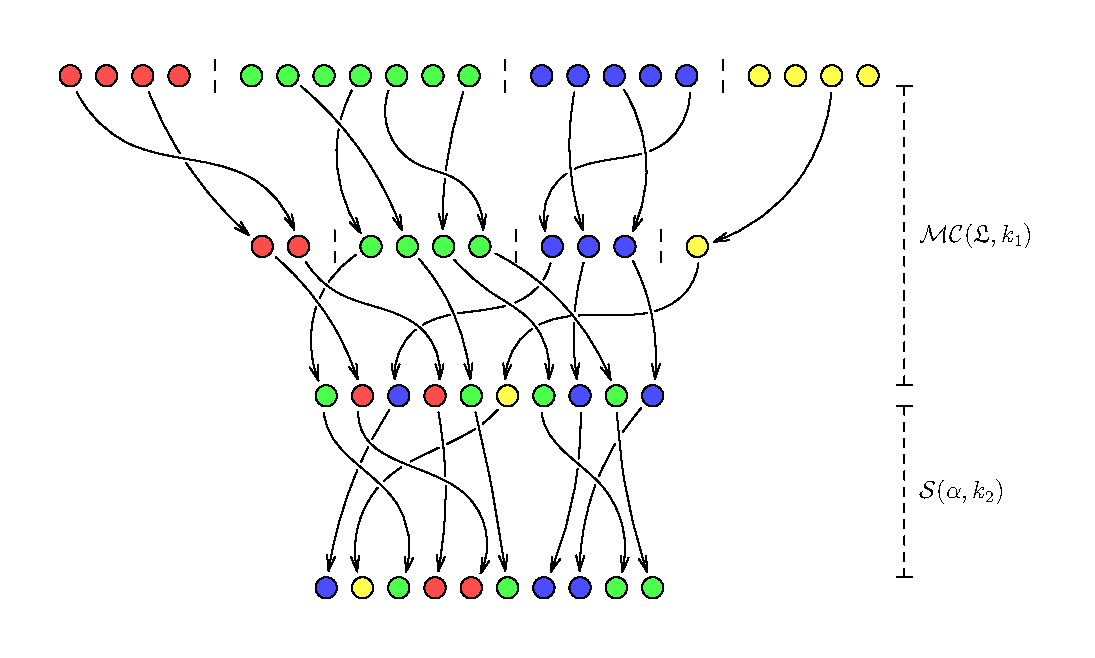
\includegraphics{figures/hash.pdf}
    \caption{An illustration of the working of the hash function}
    \label{fig:hash}
\end{figure}
%|fig|[figures/hash.asy]

\subsection{Producing different hashes with the same private keys}

The premise of this entire discussion was that one requires many passwords for different purposes. Right now, the only way is to create a new primary-secondary key pair for every new occasion. Considering how large these numbers tend to be, you may as well try to remember the hashes themselves. This is where the public key comes into play. The public key, denoted $ p $, is an integer number defined by the environment and available to the public. We will assume that it is the name of the website for which we require a password, like \texttt{"google"}, for example, converted into a number by treating the characteers in the string as digits in base-128. This number acts on the choice private key by shifting it modulo $ \#^{\M\C}(\conf) $:
\[ k_1' = \lui{\#^{\M\C}(\conf)}(k_1 + p), \] 
and then this new choice key is plugged into the hash function along with the shuffle key. Due to the injectivity of $ \H $ with respect to $ k_1 $, we see that different public keys produce different output hashes, as long as they remain in the interval $ \left( \#^{\M\C}(\conf) \right) $. Its influence on $ k_1 $ is simple and predictable, but it doesn't have to be complex, since the public key is not directly responsible for any encryption. Instead it is designed to be easily remembered.

\subsection{Counting ages of the Universe}

In this subsection, we will use a specific source configuration $ \conf $, particularly the following:

\begin{center}
\def\arraystretch{1.2}
\begin{tabular}{l|l|l|l}\ttfamily
    $ i $ & $ E_i $ & $ n_i $ & $ m_i $\\
    \hline
    0 & \ttfamily"ckapzfitqdxnwehrolmbyvsujg" & 26 & 10\\
    1 & \ttfamily"RQLIANBKJYVWPTEMCZSFDOGUHX" & 26 & 10\\
    2 & \ttfamily"=!*@?\$\%\#\&-\^{}+"        & 12 & 5\\
    3 & \ttfamily"1952074386"                 & 10 & 5\\
\end{tabular}
\end{center}

% Therefore, every password produced with this configuration will contain a total of 30 symbols, 10, 10, 5 and 5 from their respective categories.
%
% Now, let's imagine that you have inserted your two private keys into the function and got a password out of it. A sophisticated hacker sets their mind to crack your password whatever it takes. They are very smart and they have a supercomputer that can perform 1,000,000,000,000 password checks in a second, or one picosecond to check one password or key. What's more, they got their hands on the hash function and the configuration you use, so they can try to reverse-engineer your password.
%
% First, they read into the configuration and see the structure of the password. They decide to brute-force it by checking every relevant combination of 30 symbols. Well, they will have to check $ \#^{\H}(\conf) $ combinations, which in our case equals exactly
% \[ \#^{\H}(\conf) = 1,493,683,548,205,755,958,753,683,829,702,969,075,433,472,000,000,000. \] 
%
% Cracking it would take the supercomputer about $ 47,331,975,441,914,340,970,572,896,272,384 $ years, or about 3 billion of millions of millions of ages of the Universe.\\
%
% Okay, thinks the hacker, no luck. They dig a little deeper into the algorithm and find that your password depens on two private keys. The number of all pairs of such keys is
%
% \[
% \#^{(k_1,k_2)}(\conf) = \begin{array}[t]{l}
%     283,235,154,137,060,638,511,193,623,530,464,\\
%     898,307,082,375,546,273,792,000,000,000,000,000
% \end{array}
% \]
%
% This one is going to take billions of billions times longer than the previous one.\\
%
% Okay, thinks the hacker, the night is young. They are able to get their hands on one of your 30-symbol passwords because of a security leak on the website you were registered to. They have also dug ears deep into the hash function and understood how it works to the tiniest detail. Now, they want to retrieve your private keys to be able to generate your passwords to all other websites and services you use. They see that your password starts with a \texttt{'W'}. They know it was shuffled from some other position by the shuffle function, $ \S(-, k_2) $, but they don't know what the password was before the shuffling. What they do know is that your password is produced by
% \[ \#^{\cap}(\conf) = 189,621,927,936,000,000 \]
% different $ (k_1, k_2) $ pairs. The hacker now has essentially two options:



\end{document}


% = \frac{\#^{(k_1,k_2)}}{\#^{\cap}(\conf)} = \frac{\prod\limits_{i = 0}^{N-1} (n_i \mid m_i)! \cdot \left(\sum\nolimits_{i = 0}^{N-1} m_i\right)!}{\prod\limits_{i = 0}^{N-1} (m_i)!}
% Since there are $ m_i! $ ways to reorder every sub-list chosen by $ \CC $ from $ E_i $, the amount of lost information accounts for a total of $ \prod_{i = 0}^{N-1} (m_i!) $, which will be denoted by $ \#^{\cap}(\conf) $. It is the number of pairs $ (k_1, k_2) $ that produce the exact same hash. Hence, we see that the number of possible outputs of the hash function, given a configuration $ \conf $, is
